\chapter{FPGAs als Beschleuniger}\label{fpga}

Konzeption und Aufbau der \gls{fpga}s sowie der zugehörige Entwicklungsprozess
werden in diesem Kapitel geschildert. Dabei wird auf die Vorteile der
High"=Level"=Synthese gegenüber dem hardwarenahen Schaltungsentwurf auf der
Register"=Transfer"=Ebene ebenso eingegangen wie auf die bei FPGAs möglichen
Parallelisierungskonzepte.

\section{Überblick}\label{fpga:ueberblick}

Für das Verständnis der Funktionsweise eines \gls{fpga}s ist es notwendig, die
zugrunde liegenden Konzepte in Abgrenzung zu herkömmlicher Hardware
darzustellen. Dieser Abschnitt definiert zunächst den \gls{fpga}-Begriff und
erläutert im Anschluss daran den Aufbau moderner \gls{fpga}-Architekturen sowie
traditionelle und neuartige Nutzungsmöglichkeiten dieses Hardware-Typus.

\subsection{Definition}\label{fpga:ueberblick:definition}

\textit{Field-programmable gate arrays} sind, wie der Name andeutet,
konzeptionell mit den \textit{gate arrays} verwandt.

Die klassischen \textit{gate arrays} sind eine Untergruppe der integrierten
Schaltkreise (engl. \textit{integrated circuits}, IC) und gehören zur Gattung
der anwendungsspezifischen ICs (engl. \textit{application specific IC}, ASIC).
Unter ASICs versteht man jene Chips, die bereits bei der Herstellung mit einer
kundenspezifischen Schaltung versehen werden. Innerhalb dieser Kategorie gehören
\textit{gate arrays} zu den teil-vorgefertigten ASICs (engl.
\textit{semi-custom ASIC}). Diese werden zunächst in großer Menge mit demselben
technischen Grundgerüst produziert und erst in einem späteren
Herstellungsschritt in kleineren Mengen mit kundenspezifischen Schaltungen
versehen. Im Gegensatz zu ASICs, die von Anfang an nach Kundenwunsch hergestellt
wurden (engl. \textit{full-custom ASIC}), lässt sich so -- unter Inkaufnahme
geringerer erreichbarer Taktraten und schlechterer Energieeffizienz -- eine
Reduktion der Produktionskosten erreichen. \cite[vgl.][123]{kesel2013}

Allerdings haben \textit{gate arrays} den Nachteil, dass sie nur vom Hersteller
programmiert werden können. Eine Anpassung der Schaltung \glqq im Feld\grqq\
(engl. \textit{field-programmable}) ist damit nicht möglich. Mit
\gls{fpga}s wurde dieses Problem in den 1980er Jahren gelöst, indem man aus
Gattern (engl. \textit{gates}) bestehende Logikzellen von geringer Komplexität
in einer regelmäßigen Feldstruktur (engl. \textit{array}) anordnete und über
programmierbare Verdrahtungen miteinander verband. FPGAs wurden traditionell
vornehmlich im Schaltungsentwurf eingesetzt, finden mittlerweile jedoch auch in
anderen Gebieten zunehmend Verwendung (siehe
Abschnitt~\ref{fpga:ueberblick:anwendungen}).
\cite[vgl.][208]{kesel2013} 

Mittlerweile gibt es viele verschiedene \gls{fpga}-Varianten, die jedoch einige
Gemeinsamkeiten aufweisen. \gls{fpga}s bestehen stets aus einem Feld aus
Blockzellen, die so konfiguriert werden, dass sie eine bestimmte Funktion
ausführen. Diese Blockzellen integrieren durch ein dediziertes Verbindungsnetz
Logikgatter und Speicher. Dabei lassen sich vier zentrale Strukturen
unterscheiden:
\begin{itemize}
    \item Konfigurierbare Logikblöcke,
    \item programmierbare Verbindungen,
    \item Puffer für die Ein- und Ausgabe (engl. \textit{input/output}, I/O) und
    \item weitere Elemente (Speicher, arithmetische Einheiten, Taktnetzwerke,
          usw.).
\end{itemize}
In Abbildung~\ref{fpga:definition:aufbau} ist eine abstrakte \gls{fpga}-Struktur
dargestellt, die aus Logikblöcken, Verbindungen, I/O-Puffern und speziellen
Speicher- und Multiplizierer-Blöcken aufgebaut ist.
\cite[vgl.][10-13--10-14]{hawkins2010}

\begin{figure}[htb]
    \centering
    \begin{tikzpicture}
        % (0,0) ist unten links

        % untere E/A-Reihe
        \draw [fill = HKS41!60]
                (0.0, -1.875) rectangle (1.5, -1.125)
                node[pos = 0.5, text = white, align = center] {\small I/O};
        \draw [fill = HKS41!60]
                (2.625, -1.875) rectangle (4.125, -1.125)
                node[pos = 0.5, text = white, align = center] {\small I/O};
        \draw [fill = HKS41!60]
                (5.25, -1.875) rectangle (6.75, -1.125)
                node[pos = 0.5, text = white, align = center] {\small I/O};
        \draw [fill = HKS41!60]
                (7.875, -1.875) rectangle (9.375, -1.125)
                node[pos = 0.5, text = white, align = center] {\small I/O};

        % Reihe 1
        \draw [fill = HKS41!60]
                (-1.875, 0.0) rectangle (-1.125, 1.5)
                node[pos = 0.5, text = white, align = center] {\small I/O};
        \draw [fill = HKS41!80]
                (0.0, 0.0) rectangle (1.5, 1.5)
                node[pos = 0.5, text = white, align = center] {\small Logik};
        \draw [fill = HKS41!40]
                (2.625, 0.0) rectangle (4.125, 1.5)
                node[pos = 0.5, text = white, align = center] {\small Speicher};
        \draw [fill = HKS41!80]
                (5.25, 0.0) rectangle (6.75, 1.5)
                node[pos = 0.5, text = white, align = center] {\small Logik};
        \draw [fill = HKS41]
                (7.875, 0.0) rectangle (9.375, 1.5)
                node[pos = 0.5, text = white, align = center] {\small Multipli- \\ zierer};
        \draw [fill = HKS41!60]
                (10.5, 0.0) rectangle (11.25, 1.5)
                node[pos = 0.5, text = white, align = center] {\small I/O};

        % Reihe 2
        \draw [fill = HKS41!60]
                (-1.875, 2.625) rectangle (-1.125, 4.125)
                node[pos = 0.5, text = white, align = center] {\small I/O};
        \draw [fill = HKS41!80]
                (0.0, 2.625) rectangle (1.5, 4.125)
                node[pos = 0.5, text = white, align = center] {\small Logik};
        \draw [fill = HKS41!40]
                (2.625, 2.625) rectangle (4.125, 4.125)
                node[pos = 0.5, text = white, align = center] {\small Speicher};
        \draw [fill = HKS41!80]
                (5.25, 2.625) rectangle (6.75, 4.125)
                node[pos = 0.5, text = white, align = center] {\small Logik};
        \draw [fill = HKS41]
                (7.875, 2.625) rectangle (9.375, 4.125)
                node[pos = 0.5, text = white, align = center] {\small Multipli- \\ zierer};
        \draw [fill = HKS41!60]
                (10.5, 2.625) rectangle (11.25, 4.125)
                node[pos = 0.5, text = white, align = center] {\small I/O};

        % Reihe 3
        \draw [fill = HKS41!60]
                (-1.875, 5.25) rectangle (-1.125, 6.75)
                node[pos = 0.5, text = white, align = center] {\small I/O};
        \draw [fill = HKS41!80]
                (0.0, 5.25) rectangle (1.5, 6.75)
                node[pos = 0.5, text = white, align = center] {\small Logik};
        \draw [fill = HKS41!40]
                (2.625, 5.25) rectangle (4.125, 6.75)
                node[pos = 0.5, text = white, align = center] {\small Speicher};
        \draw [fill = HKS41!80]
                (5.25, 5.25) rectangle (6.75, 6.75)
                node[pos = 0.5, text = white, align = center] {\small Logik};
        \draw [fill = HKS41]
                (7.875, 5.25) rectangle (9.375, 6.75)
                node[pos = 0.5, text = white, align = center] {\small Multipli- \\ zierer};
        \draw [fill = HKS41!60]
                (10.5, 5.25) rectangle (11.25, 6.75)
                node[pos = 0.5, text = white, align = center] {\small I/O};

        % Reihe 3
        \draw [fill = HKS41!60]
                (-1.875, 7.875) rectangle (-1.125, 9.375)
                node[pos = 0.5, text = white, align = center] {\small I/O};
        \draw [fill = HKS41!80]
                (0.0, 7.875) rectangle (1.5, 9.375)
                node[pos = 0.5, text = white, align = center] {\small Logik};
        \draw [fill = HKS41!40]
                (2.625, 7.875) rectangle (4.125, 9.375)
                node[pos = 0.5, text = white, align = center] {\small Speicher};
        \draw [fill = HKS41!80]
                (5.25, 7.875) rectangle (6.75, 9.375)
                node[pos = 0.5, text = white, align = center] {\small Logik};
        \draw [fill = HKS41]
                (7.875, 7.875) rectangle (9.375, 9.375)
                node[pos = 0.5, text = white, align = center] {\small Multipli- \\ zierer};
        \draw [fill = HKS41!60]
                (10.5, 7.875) rectangle (11.25, 9.375)
                node[pos = 0.5, text = white, align = center] {\small I/O};

        % obere E/A-Reihe
        \draw [fill = HKS41!60]
                (0.0, 10.5) rectangle (1.5, 11.25)
                node[pos = 0.5, text = white, align = center] {\small I/O};
        \draw [fill = HKS41!60]
                (2.625, 10.5) rectangle (4.125, 11.25)
                node[pos = 0.5, text = white, align = center] {\small I/O};
        \draw [fill = HKS41!60]
                (5.25, 10.5) rectangle (6.75, 11.25)
                node[pos = 0.5, text = white, align = center] {\small I/O};
        \draw [fill = HKS41!60]
                (7.875, 10.5) rectangle (9.375, 11.25)
                node[pos = 0.5, text = white, align = center] {\small I/O};

        % Verbindungen - Spalte 1
        \draw [color = HKS92!90, line width = 5mm]
                (0.75, -1.125) -- (0.75, 0.0);
        \draw [color = HKS92!90, line width = 5mm]
                (0.75, 1.5) -- (0.75, 2.625);
        \draw [color = HKS92!90, line width = 5mm]
                (0.75, 4.125) -- (0.75, 5.25);
        \draw [color = HKS92!90, line width = 5mm]
                (0.75, 6.75) -- (0.75, 7.875);
        \draw [color = HKS92!90, line width = 5mm]
                (0.75, 9.375) -- (0.75, 10.5);

        % Verbindungen - Spalte 2
        \draw [color = HKS92!90, line width = 5mm]
                (3.375, -1.125) -- (3.375, 0.0);
        \draw [color = HKS92!90, line width = 5mm]
                (3.375, 1.5) -- (3.375, 2.625);
        \draw [color = HKS92!90, line width = 5mm]
                (3.375, 4.125) -- (3.375, 5.25);
        \draw [color = HKS92!90, line width = 5mm]
                (3.375, 6.75) -- (3.375, 7.875);
        \draw [color = HKS92!90, line width = 5mm]
                (3.375, 9.375) -- (3.375, 10.5);

        % Verbindungen - Spalte 3
        \draw [color = HKS92!90, line width = 5mm]
                (6.0, -1.125) -- (6.0, 0.0);
        \draw [color = HKS92!90, line width = 5mm]
                (6.0, 1.5) -- (6.0, 2.625);
        \draw [color = HKS92!90, line width = 5mm]
                (6.0, 4.125) -- (6.0, 5.25);
        \draw [color = HKS92!90, line width = 5mm]
                (6.0, 6.75) -- (6.0, 7.875);
        \draw [color = HKS92!90, line width = 5mm]
                (6.0, 9.375) -- (6.0, 10.5);

        % Verbindungen - Spalte 4
        \draw [color = HKS92!90, line width = 5mm]
                (8.625, -1.125) -- (8.625, 0.0);
        \draw [color = HKS92!90, line width = 5mm]
                (8.625, 1.5) -- (8.625, 2.625);
        \draw [color = HKS92!90, line width = 5mm]
                (8.625, 4.125) -- (8.625, 5.25);
        \draw [color = HKS92!90, line width = 5mm]
                (8.625, 6.75) -- (8.625, 7.875);
        \draw [color = HKS92!90, line width = 5mm]
                (8.625, 9.375) -- (8.625, 10.5);

        % Verbindungen - Reihe 1
        \draw [color = HKS92!90, line width = 5mm]
                (-1.125, 0.75) -- (0.0, 0.75);
        \draw [color = HKS92!90, line width = 5mm]
                (1.5, 0.75) -- (2.625, 0.75);
        \draw [color = HKS92!90, line width = 5mm]
                (4.125, 0.75) -- (5.25, 0.75);
        \draw [color = HKS92!90, line width = 5mm]
                (6.75, 0.75) -- (7.875, 0.75);
        \draw [color = HKS92!90, line width = 5mm]
                (9.375, 0.75) -- (10.5, 0.75);

        % Verbindungen - Reihe 2
        \draw [color = HKS92!90, line width = 5mm]
                (-1.125, 3.375) -- (0.0, 3.375);
        \draw [color = HKS92!90, line width = 5mm]
                (1.5, 3.375) -- (2.625, 3.375);
        \draw [color = HKS92!90, line width = 5mm]
                (4.125, 3.375) -- (5.25, 3.375);
        \draw [color = HKS92!90, line width = 5mm]
                (6.75, 3.375) -- (7.875, 3.375);
        \draw [color = HKS92!90, line width = 5mm]
                (9.375, 3.375) -- (10.5, 3.375);

        % Verbindungen - Reihe 3
        \draw [color = HKS92!90, line width = 5mm]
                (-1.125, 6.0) -- (0.0, 6.0);
        \draw [color = HKS92!90, line width = 5mm]
                (1.5, 6.0) -- (2.625, 6.0);
        \draw [color = HKS92!90, line width = 5mm]
                (4.125, 6.0) -- (5.25, 6.0);
        \draw [color = HKS92!90, line width = 5mm]
                (6.75, 6.0) -- (7.875, 6.0);
        \draw [color = HKS92!90, line width = 5mm]
                (9.375, 6.0) -- (10.5, 6.0);

        % Verbindungen - Reihe 4
        \draw [color = HKS92!90, line width = 5mm]
                (-1.125, 8.625) -- (0.0, 8.625);
        \draw [color = HKS92!90, line width = 5mm]
                (1.5, 8.625) -- (2.625, 8.625);
        \draw [color = HKS92!90, line width = 5mm]
                (4.125, 8.625) -- (5.25, 8.625);
        \draw [color = HKS92!90, line width = 5mm]
                (6.75, 8.625) -- (7.875, 8.625);
        \draw [color = HKS92!90, line width = 5mm]
                (9.375, 8.625) -- (10.5, 8.625);

        % Verbindungen - Zwischenspalten
        \draw [color = HKS92!90, line width = 5mm]
                (-0.5625, -0.8125) -- (-0.5625, 10.1875);
        \draw [color = HKS92!90, line width = 5mm]
                (2.0625, -0.5625) -- (2.0625, 9.9375);
        \draw [color = HKS92!90, line width = 5mm]
                (4.6875, -0.5625) -- (4.6875, 9.9375);
        \draw [color = HKS92!90, line width = 5mm]
                (7.3125, -0.5625) -- (7.3125, 9.9375);
        \draw [color = HKS92!90, line width = 5mm]
                (9.9375, -0.8125) -- (9.9375, 10.1875);

        % Verbindungen - Zwischenzeilen
        \draw [color = HKS92!90, line width = 5mm]
                (-0.5625, -0.5625) -- (9.9375, -0.5625);
        \draw [color = HKS92!90, line width = 5mm]
                (-0.5625, 2.0625) -- (9.9375, 2.0625);
        \draw [color = HKS92!90, line width = 5mm]
                (-0.5625, 4.6875) -- (9.9375, 4.6875);
        \draw [color = HKS92!90, line width = 5mm]
                (-0.5625, 7.3125) -- (9.9375, 7.3125);
        \draw [color = HKS92!90, line width = 5mm]
                (-0.5625, 9.9375) -- (9.9375, 9.9375);
    \end{tikzpicture}
    \caption{abstrakter FPGA-Aufbau \cite[nach][10-14]{hawkins2010}}
    \label{fpga:definition:aufbau}
\end{figure}

\subsection{Aufbau moderner FPGAs}\label{fpga:ueberblick:aufbau}

Am Beispiel der Virtex"=UltraScale+"=Architektur der Firma Xilinx soll der
Aufbau eines modernen \gls{fpga} verdeutlicht werden. \gls{fpga}s dieser
Architektur bestehen aus sechs fundamentalen programmierbaren Elementen:
\begin{itemize}
    \item Konfigurierbare Logikblöcke (engl. \gls{clb}) bestehen aus acht
          Logikeinheiten, die man als \gls{lut} bezeichnet und zur
          Generierung von Logikfunktionen verwendet werden können. Daneben sind
          in einem \gls{clb} Speicherelemente enthalten, die als Flip"=Flop oder
          Latch verwendet werden können, sowie weitere Elemente wie Multiplexer
          oder Einheiten für den arithmetischen Übertrag.
          \cite[vgl.][6]{ultrascaleclb2017}
    \item Eingabe/Ausgabe-Blöcke (engl. \gls{iob}) werden zur Steuerung des
          Datenflusses zwischen den E/A-Pins und der internen Schaltkreise
          benutzt. Die UltraScale+-Architektur bietet verschiedene
          \gls{iob}-Typen, die z.B. verschiedene E/A-Standards oder uni- oder
          bidirektionale Kommunikation unterstützen. \cite[vgl. die
          ausführliche E/A"=Beschreibung in][Kapitel 1 und 2]{ultrascaleio2019}
    \item \glqq Block RAM\grqq\ kann bis zu \SI{36}{\kilo\bit} speichern. Dabei
          lässt sich ein Block bei Bedarf auch in zwei unabhängige RAMs mit
          jeweils \SI{18}{\kilo\bit} zerlegen. Zusätzlich sind in einem
          Taktschritt voneinander unabhängige Lese- und Schreibzugriffe möglich.
          Benachbarte Blöcke lassen sich darüber hinaus miteinander verbinden,
          um größere RAM-Bereiche zu generieren.
          \cite[vgl.][6]{ultrascalemem2019}
    \item UltraRAM-Blöcke können bis zu \SI{288}{\kilo\bit} speichern, sind im
          Vergleich mit Block RAM aber unflexibler, da Lese- und Schreibzugriffe
          nicht parallel in einem Taktschritt möglich sind. Wie beim Block RAM
          lassen sich auch beim UltraRAM mehrere Blöcke zusammenschalten, um
          einen größeren Speicher zu erzeugen.
          \cite[vgl.][92--94]{ultrascalemem2019}
    \item Digitale Signalprozessoren (engl. \gls{dsp}) sind Blöcke, die für die
          Ausführung fundamentaler mathematischer oder bitweiser Operationen der
          Signal-, Bild- und Videoverarbeitung besonders gut geeignet sind. Aus
          mehreren \gls{dsp}s lassen sich durch Verbindungen komplexere
          arithmetische Funktionen generieren.
          \cite[vgl.][7--8]{ultrascaledsp2019}
    \item Blöcke für die Taktverwaltung (engl. \gls{cmt}) generieren den Takt
          für die restlichen Komponenten des \gls{fpga}. Sie sind ebenso dazu
          geeignet, Operationen auf einem von außen kommenden Takt
          durchzuführen, z.B. eine Phasenverschiebung oder eine Filterung.
          \cite[vgl.][35--40]{ultrascaleclock2018}
\end{itemize}

Sollen FPGAs als Beschleuniger zum Einsatz kommen, ist die Verwendung weiterer
Hardware"=Komponenten sinnvoll. Diese befinden sich zwar auf derselben Platine
wie der eigentliche FPGA, aber nicht auf demselben Chip. Dies trifft z.B. auf
den als DRAM bezeichneten Off"=Chip"=Speicher zu, der mehrere \si{\gibi\byte}
umfassen kann. Im Vergleich zu Block RAM und UltraRAM weist dieser Speichertyp
aber deutlich geringere Speicherbandbreiten auf. Auf dem Beschleuniger
\textit{Alveo U200}, der mit einem UltraScale+-\gls{fpga} mit der
Modellbezeichnung \textit{XCU200} ausgestattet ist, finden sich beispielsweise
vier DDR4-RAM-Module mit einer Bandbreite von \SI{77}{\gibi\byte\per\second}
\cites[vgl.][3]{alveo2019}[2]{alveobrief2018}. Weitere typische Bestandteile
eines Beschleunigers sind z.B. eine Schnittstelle zur CPU und dem Hauptspeicher
des Gesamtsystems (etwa über PCI Express) oder Komponenten für die Energieverwaltung.

Ein XCU200-\gls{fpga} verteilt die oben genannten programmierbaren
On"=Chip"=Elemente auf drei Abschnitte, die als \gls{slr} bezeichnet werden.
Gemeinsam bilden die \gls{slr}s drei dynamische Regionen sowie eine statische
Region, die alle mit dem DRAM des Beschleunigers verbunden sind
(siehe Abbildung~\ref{fpga:aufbau:alveoslr}). Die dynamischen Regionen lassen
sich vom Benutzer konfigurieren, während die statische Region der
Laufzeitumgebung des \gls{fpga}-Host-Systems vorbehalten ist
\cite[vgl.][4]{alveo2019}. Die Ressourcen verteilen sich in unterschiedlicher
Anzahl auf die \gls{slr}s, wie Tabelle~\ref{fpga:aufbau:ressourcen} zeigt.

\begin{figure}[htb]
    \centering
    \begin{tikzpicture}
        % unten
        \draw (0.0, 0.0) rectangle (7.5, 2.5)
            node [pos = 0.5] {dynamische Region}
            node [pos = 0.1] {SLR0};

        % Mitte
        \draw [draw = none] (0.0, 2.5) rectangle (7.5, 5)
            node [pos = 0.1] {SLR1};
        \draw (0.0, 2.5) rectangle (3.75, 5)
            node [pos = 0.5] {dynamische Region};
        \draw [fill = HKS92!90] (3.75, 2.5) rectangle (7.5, 5)
            node [pos = 0.5, color = white] {statische Region};

        % oben
        \draw (0.0, 5) rectangle (7.5, 7.5)
            node [pos = 0.5] {dynamische Region}
            node [pos = 0.1] {SLR2};
    \end{tikzpicture}
    \caption{Aufbau eines XCU200-FPGAs \cite[nach][5]{alveo2019}}
    \label{fpga:aufbau:alveoslr}
\end{figure}

\begin{table}[htb]
    \centering
    \begin{tabulary}{\textwidth}{@{}LCCCC@{}}
        \toprule
        \textbf{Ressource} & \textbf{Gesamt} & \textbf{SLR0} & \textbf{SLR1}
            & \textbf{SLR2} \tabularnewline\midrule
        CLB & \num{111500} & \num{45625} & \num{20250} &
            \num{45625}\tabularnewline
        Block RAM (\SI{36}{\kibi\byte}) & \num{1766} & \num{695} & 
            \num{376} & \num{695}\tabularnewline
        UltraRAM (\SI{288}{\kibi\byte}) & \num{800} & \num{320} &
            \num{160} & \num{320}\tabularnewline
        DSP & \num{5867} & \num{2275} & \num{1317} &
            \num{2275}\tabularnewline\bottomrule
    \end{tabulary}
    \caption{Ressourcen der dynamischen Regionen eines XCU200-FPGAs
             \cite[siehe][5]{alveo2019}}
    \label{fpga:aufbau:ressourcen}
\end{table}

Innerhalb der \gls{slr}s sind die Ressourcen spaltenweise verteilt (wie in
Abbildung~\ref{fpga:aufbau:spalten} dargestellt). Zusätzlich werden die Spalten
in vertikale Abschnitte von 60 \gls{clb}s bzw. der äquivalenten Anzahl der
anderen Blocktypen unterteilt. Ein solcher Abschnitt bildet eine von Xilinx als
\textit{clock region} bezeichnete Struktur. Zusammengefasst ergibt sich
dadurch eine spaltenorientierte Gitterstruktur, wie sie in
Abbildung~\ref{fpga:aufbau:clockregions} zu sehen ist.
\cite[vgl.][22]{ultrascale2019}

\begin{figure}[htb]
    \centering
    \begin{tikzpicture}
        \draw [fill = HKS92!90] (0.0, 0.0) rectangle (1.0, 8.0)
            node [pos = 0.5, rotate = 90, color = white] {externe E/A};
        \draw (1.0, 0.0) rectangle (2.5, 8.0)
            node [pos = 0.5, rotate = 90] {CLB, DSP, Block RAM, UltraRAM};
        \draw [fill = HKS92!70] (2.5, 0.0) rectangle (3.5, 8.0)
            node [pos = 0.5, rotate = 90, color = white] {E/A, Takt, Speicherschnittstelle};
        \draw (3.5, 0.0) rectangle (5.0, 8.0)
            node [pos = 0.5, rotate = 90] {CLB, DSP, Block RAM, UltraRAM};
        \draw [fill = HKS92!70] (5.0, 0.0) rectangle (6.0, 8.0)
            node [pos = 0.5, rotate = 90, color = white] {E/A, Takt, Speicherschnittstelle};
        \draw (6.0, 0.0) rectangle (7.5, 8.0)
            node [pos = 0.5, rotate = 90] {CLB, DSP, Block RAM, UltraRAM};
        \draw [fill = HKS92!90] (7.5, 0.0) rectangle (8.5, 8.0)
            node [pos = 0.5, rotate = 90, color = white] {externe E/A};
    \end{tikzpicture}
    \caption{spaltenweise Verteilung der FPGA-Ressourcen
             \cite[nach][22]{ultrascale2019}}
    \label{fpga:aufbau:spalten}
\end{figure}

\begin{figure}[htb]
    \centering
    \begin{tikzpicture}
        % Spalten
        \draw [fill = HKS92!90] (0.0, 0.0) rectangle (1.0, 8.0);
        \draw (1.0, 0.0) rectangle (2.5, 8.0);
        \draw [fill = HKS92!70] (2.5, 0.0) rectangle (3.5, 8.0);
        \draw (3.5, 0.0) rectangle (5.0, 8.0);
        \draw [fill = HKS92!70] (5.0, 0.0) rectangle (6.0, 8.0);
        \draw (6.0, 0.0) rectangle (7.5, 8.0);
        \draw [fill = HKS92!90] (7.5, 0.0) rectangle (8.5, 8.0);

        % Querlinien
        \draw (0.0, 2.0) -- (8.5, 2.0);
        \draw (0.0, 4.0) -- (8.5, 4.0);
        \draw (0.0, 6.0) -- (8.5, 6.0);

        % Klammer
        \draw [decorate, decoration = {brace, amplitude = 2.5mm}, xshift = -2mm]
            (0.0, 6.0) -- (0.0, 8.0)
            node [pos = 0.5, xshift = -11mm, align = center] {60 CLBs};
    \end{tikzpicture}
    \caption{Aufteilung der FPGA-Ressourcen auf \textit{clock regions}
             \cite[nach][22]{ultrascale2019}}
    \label{fpga:aufbau:clockregions}
\end{figure}

\subsection{Anwendungsfälle}\label{fpga:ueberblick:anwendungen}

Gegenüber ASICs bieten \gls{fpga}s einige Vorteile. Da sich Schaltungen ohne
einen Produktionsprozess schneller in Hardware abbilden lassen, eignen sich
\gls{fpga}s für die Entwicklung neuer Schaltungen durch die Methode des
\textit{rapid prototyping} und damit für eine schnellere Markteinführung. Durch
die einfache Neuprogrammierung lassen sich Fehler außerdem während des
Entwicklungsprozesses sowie während des Lebenszyklus des Produkts deutlich
einfacher beheben, als dies bei ASICs der Fall wäre.
\cite[vgl.][10-1]{hawkins2010}

Dadurch eignen sich \gls{fpga}s sehr gut für den Einsatz als Schaltkreise, die
in kleiner bis mittlerer Stückzahl produziert werden sollen, weil die
finanzielle Einstiegshürde deutlich geringer als bei ASICs ist. Umgekehrt sind
ASICs bei hohen Produktionsvolumen überlegen, da die Kosten pro Chip geringer
sind.
\cite[vgl.][10-2]{hawkins2010}

In jüngerer Zeit wurden \gls{fpga}s auch außerhalb des klassischen
Schaltkreisentwurfs eingesetzt. So setzt die Firma Microsoft beispielsweise
\gls{fpga}s des Herstellers Intel für die Inferenz tiefer neuraler Netzwerke
\cite[vgl.][]{fowers2018, chung2018} sowie als besonders schnelle
Netzwerkkarten ein \cite[vgl.][]{firestone2018}. Der Cloud"=Anbieter Amazon
bietet spezielle FPGA"=Instanzen an, in denen Xilinx"=FPGAs als Beschleuniger
genutzt werden können \cite[vgl.][]{amazonec2f1}, wovon in der Literatur bereits
Gebrauch gemacht wurde \cite[vgl. etwa][]{ditucci2017}.

\section{Entwicklungsprozess}\label{fpga:entwicklung}

Es sind bei der Software"=Entwicklung für \gls{fpga}s zwei Vorgehensweisen
voneinander abzugrenzen: Einerseits die Entwicklung durch
Hardware"=Beschreibungssprachen (in dieser Arbeit nur kurz skizziert) und
andererseits die High"=Level"=Synthese, die auf in Hochsprachen implementierten
Algorithmen basiert. Die Ansätze unterscheiden sich durch ihre Abstraktion der
zugrunde liegenden Hardware (die verschiedenen Abstraktionsebenen wurden von
Gajski in seinem Y"=Diagramm zusammengefasst, siehe
Abbildung~\ref{fpga:entwicklung:ydiagramm}). Die Hardware"=Beschreibungssprachen
befinden sich mit der Register"=Transfer"=Ebene auf einem hardware"=nahen Level
und Detaillierungsgrad, während die Hochsprachene auf der algorithmischen
oder der Systemebene anzusiedeln sind. \cite[vgl.][10--11]{kesel2013}

\begin{figure}[htb]
    \centering
    \begin{tikzpicture}
        % Kreise
        \draw [postaction = {decorate,
                             decoration = {text along path,
                                           raise = 1mm,
                                           text align = {align = center,
                                                         left indent = 3.15cm},
                                           text = {|\fontsize{6.5}{7.8}\selectfont|Transistorebene},
                                           reverse path}}]
              (0, 0) circle [radius = 1.0];

        \draw [postaction = {decorate,
                             decoration = {text along path,
                                           raise = 1mm,
                                           text align = {align = center,
                                                         left indent = 6.3cm},
                                           text = {|\small|Gatterebene},
                                           reverse path}}]
              (0, 0) circle [radius = 2.0];

        \draw [postaction = {decorate,
                             decoration = {text along path,
                                           raise = 1mm,
                                           text align = {align = center,
                                                         left indent = 9.45cm},
                                           text = {|\small|Register-Transfer-Ebene},
                                           reverse path}}]
              (0, 0) circle [radius = 3.0];

        \draw [postaction = {decorate,
                             decoration = {text along path,
                                           raise = 1mm,
                                           text align = {align = center,
                                                         left indent = 12.6cm},
                                           text = {|\small|Algorithmische Ebene},
                                           reverse path}}]
              (0, 0) circle [radius = 4.0];

        \draw [postaction = {decorate,
                             decoration = {text along path,
                                           raise = 1mm,
                                           text align = {align = center,
                                                         left indent = 15.75cm},
                                           text = {|\small|Systemebene},
                                           reverse path}}]
              (0, 0) circle [radius = 5.0];

        % Linien
        \draw [thick] (0, 0) -- (30:6cm) node [pos = 1.125, sloped] {\small Struktur};
        \draw [thick] (0, 0) -- (150:6cm) node [pos = 1.15, sloped] {\small Verhalten};
        \draw [thick] (0, 0) -- (270:6cm) 
              node [pos = 1.05] {\small Geometrie / Physikalische Implementierung};

        % Schnittpunkte
        \draw [fill = HKS92!90] (30:1cm) circle [radius = 0.15]
              node [below right, xshift = 2mm, fill = white, inner sep = 1pt, rotate = -30]
                   {\fontsize{6.5}{7.8}\selectfont Transistor};
        \draw [fill = HKS92!90] (30:2cm) circle [radius = 0.15]
              node [below right, xshift = 2mm, fill = white, inner sep = 1pt, rotate = -30]
                   {\fontsize{6.5}{7.8}\selectfont Gatter, Flip"=Flop};
        \draw [fill = HKS92!90] (30:3cm) circle [radius = 0.15]
              node [below right, xshift = 2mm, fill = white, inner sep = 1pt, rotate = -30]
                   {\fontsize{6.5}{7.8}\selectfont ALU, Register};
        \draw [fill = HKS92!90] (30:4cm) circle [radius = 0.15]
              node [below right, xshift = 2mm, fill = white, inner sep = 1mm, rotate = -30]
                   {\fontsize{6.5}{7.8}\selectfont Prozessor};
        \draw [fill = HKS92!90] (30:5cm) circle [radius = 0.15]
              node [below right, xshift = 2mm, fill = white, inner sep = 1mm, rotate = -30]
                   {\fontsize{6.5}{7.8}\selectfont CPU, Speicher};

        \draw [fill = HKS92!90] (150:1cm) circle [radius = 0.15]
              node [below left, xshift = -2mm, fill = white, inner sep = 1pt, rotate = 30]
                   {\fontsize{6.5}{7.8}\selectfont Differentialgleichungen};
        \draw [fill = HKS92!90] (150:2cm) circle [radius = 0.15]
              node [below left, xshift = -2mm, fill = white, inner sep = 1pt, rotate = 30]
                   {\fontsize{6.5}{7.8}\selectfont Boolesche Gleichungen};
        \draw [fill = HKS92!90] (150:3cm) circle [radius = 0.15]
              node [below left, xshift = -2mm, fill = white, inner sep = 1pt, rotate = 30]
                   {\fontsize{6.5}{7.8}\selectfont Register-Transfer};
        \draw [fill = HKS92!90] (150:4cm) circle [radius = 0.15]
              node [below left, xshift = -2mm, fill = white, inner sep = 1pt, rotate = 30]
                   {\fontsize{6.5}{7.8}\selectfont Algorithmus};
        \draw [fill = HKS92!90] (150:5cm) circle [radius = 0.15]
              node [below left, xshift = -2mm, fill = white, inner sep = 1pt, rotate = 30]
                   {\fontsize{6.5}{7.8}\selectfont System-Spezifikation};

        \draw [fill = HKS92!90] (270:1cm) circle [radius = 0.15]
              node [right, xshift = 2mm, fill = white, inner sep = 1pt]
                   {\fontsize{6.5}{7.8}\selectfont Polygone};
        \draw [fill = HKS92!90] (270:2cm) circle [radius = 0.15]
              node [right, xshift = 2mm, fill = white, inner sep = 1pt]
                   {\fontsize{6.5}{7.8}\selectfont Zelle};
        \draw [fill = HKS92!90] (270:3cm) circle [radius = 0.15]
              node [right, xshift = 2mm, fill = white, inner sep = 1pt]
                   {\fontsize{6.5}{7.8}\selectfont Makro};
        \draw [fill = HKS92!90] (270:4cm) circle [radius = 0.15]
              node [right, xshift = 2mm, fill = white, inner sep = 1pt]
                   {\fontsize{6.5}{7.8}\selectfont Block};
        \draw [fill = HKS92!90] (270:5cm) circle [radius = 0.15]
              node [right, xshift = 2mm, fill = white, inner sep = 1pt]
                   {\fontsize{6.5}{7.8}\selectfont Chip};
    \end{tikzpicture}
    \caption{Y"=Diagramm nach Gajski \cite[nach][10]{kesel2013}}
    \label{fpga:entwicklung:ydiagramm}
\end{figure}

\subsection{Hardware-Beschreibungssprachen}\label{fpga:entwicklung:hdl}

Eine häufig verwendete Hardware"=Beschreibungssprache ist VHDL, was für
\textit{VHSIC Hardware Description Language} steht, wobei VHSIC eine Abkürzung
für \textit{Very High Speed Integrated Circuit} ist. Die Sprache geht auf ein
Programm des US"=amerikanischen Verteidigungsministerium zurück, das in den
1980er Jahren eine einheitliche Beschreibungs- bzw.\ Dokumentationssprache für
komplexe Schaltungen wünschte, und ist an die Programmiersprache Ada angelehnt.
\cite[vgl.][22]{kesel2013}

Eine weitere bekannte Beschreibungssprache ist Verilog
(\textit{Verifying Logic}), die ebenfalls in den 1980er Jahren entwickelt wurde
und an der Programmiersprache C orientiert ist. Sie wurde als ursprünglich
proprietäre Sprache von der Firma \textit{Gateway Design Automation} geschaffen
und lässt sich in ihrem Umfang mit VHDL vergleichen. Verilog ist vor allem in
den Vereinigten Staaten verbreitet, während europäische Entwickler eher auf VHDL
setzen. In den folgenden Abschnitten werden die Konzepte der
Beschreibungssprachen daher am Beispiel von VHDL erläutert.
\cite[vgl.][24--25]{kesel2013}

\subsubsection{Konzepte}

VHDL ist eine Sprache für die Hardware"=Modellierung und unterscheidet sich in
einigen wichtigen Punkten von Hochsprachen wie C++. Stehen bei Hochsprachen
die algorithmischen Aspekte im Vordergrund, ist bei VHDL entscheidend, wie der
Algorithmus in eine Hardware"=Beschreibung umgesetzt werden kann. Dabei wird die
konzeptionelle Schaltung zunächst in mehrere \textit{Komponenten} zerlegt. Die
Beschreibung jeder \textit{Komponente} erfolgt dann auf der
Register"=Transfer"=Ebene, das heißt, dass zwischen speichernden (Register) und
kombinatorischen (Transferfunktionen) Aspekten unterschieden wird. Aus der
Digitaltechnik stammt eine Darstellungsweise als \glqq endlicher Automat\grqq\
(siehe Abbildung~\ref{fpga:hdl:moore}): Die Eingabe-Transferfunktion $f$
berechnet durch die Kombination logischer Operatoren (UND, ODER, NICHT, \ldots)
aus der Eingangsvariablen $X$ und der Zustandsvariablen $Z$ des Registers den
neuen, im nächsten Takt zu übernehmenden Registerwert $Z+$. Durch die
Kombination logischer Operatoren ist $f$ eine Boolesche Funktion\footnote{auch
logische Funktion genannt}:
%
\[
    Z+ = f(X, Z)
\]
%
Die Ausgabe"=Transferfunktion $g$ berechnet die Ausgabevariable $Y$ aus $Z$ und
lässt sich ebenfalls als Boolesche Funktion darstellen:
%
\[
    Y = g(Z)
\]
%
Diese Darstellung wird auch als Moore"=Schaltwerk bezeichnet.
\cite[vgl.][34--35]{kesel2013}
%
\begin{figure}
    \centering
    \begin{tikzpicture}
        \draw [fill = HKS92!90] (0, 0)   rectangle (0.5, 0.5);
        \draw [fill = HKS92!90] (0, 1.75) rectangle (0.5, 2.25);

        \draw (1.5, 1.0) rectangle (5.0, 5.5)
                         node [pos = 0.5, align = center]
                              {\small Eingabe-\\\small Transferfunktion};
        \draw (6.5, 1.0) rectangle (8.25, 5.5)
                         node [pos = 0.5, align = center] {\small Register};
        \draw (9.75, 1.0) rectangle (13.25, 5.5)
                         node [pos = 0.5, align = center]
                              {\small Ausgabe-\\\small Transferfunktion};


        \draw [-{Latex[length = 3mm]}] (0.5, 0.25) 
                    -- (7.375, 0.25)
                       node [pos = 0.15, fill = white, inner sep = 1pt] {Takt}
                    -- (7.375, 1.0);
        \draw [-{Latex[length = 3mm]}] (0.5, 2.0) -- (1.5, 2.0) 
                    node [pos = 0.35, fill = white, inner sep = 1pt] {$X$};
        \draw [-{Latex[length = 3mm]}] (5.0, 3.25) -- (6.5, 3.25)
                    node [pos = 0.45, fill = white, inner sep = 1pt] {$Z+$};
        \draw [-{Latex[length = 3mm]}] (8.25, 3.25) -- (9.75, 3.25);
        \draw [-{Latex[length = 3mm]}] (9, 3.25)
                    -- (9, 6.0)
                    -- (0.5, 6.0)
                       node [pos = 0.4, fill = white, inner sep = 1pt] {$Z$}
                    -- (0.5, 4.5)
                    -- (1.5, 4.5);
        \draw [-{Latex[length = 3mm]}] (13.25, 3.25) -- (14.75, 3.25)
                    node [right, xshift = 1mm] {$Y$};
    \end{tikzpicture}
    \caption{Modell eines endlichen Automaten (Moore"=Schaltwerk)
             \cite[nach][35]{kesel2013}}
    \label{fpga:hdl:moore}
\end{figure}

Die Anschlüsse einer einzelnen \textit{Komponente} werden in VHDL als
\textit{Entity} bezeichnet. Sie sind notwendig, um mehrere \textit{Komponenten}
miteinander verschalten zu können. Der Quelltext~\ref{fpga:hdl:regentity} zeigt
eine \textit{Entity} für ein 2"=Bit"=Register. \cite[vgl.][25]{kesel2013}

\begin{code}
    \begin{minted}[fontsize=\small]{vhdl}
LIBRARY ieee;
USE ieee.std_logic_1164.all;

ENTITY reg2 IS
    PORT(
        clk  : IN   std_logic;
        d0   : IN   std_logic;
        d1   : IN   std_logic;
        load : IN   std_logic;
        res  : IN   std_logic;
        q0   : OUT  std_logic;
        q1   : OUT  std_logic
    );
END reg2 ;
    \end{minted}
    \caption{\textit{Entity} eines 2-Bit-Registers \cite[siehe][26]{kesel2013}}
    \label{fpga:hdl:regentity}
\end{code}

Jeder \textit{Entity} wird mindestens eine \textit{Architecture} zugeordnet.
Diese beschreibt entweder die innere Funktion, also das Verhalten, oder die
Struktur, das heißt die Verschaltung von Teil-Komponenten. Eine
\textit{Architecture} ist also entweder eine Verhaltensbeschreibung oder eine
Strukturbeschreibung. Strukturbeschreibungen können sowohl in Text- als auch
in grafischer Form (mittels spezieller Schema-Editoren) angelegt werden, während
Verhaltensbeschreibungen üblicherweise nur in Textform verfasst werden.
\cite[vgl.][27]{kesel2013}

Einer \textit{Entity} lassen sich auch mehrere unterschiedliche
\textit{Architectures} zuordnen. So lässt sich dieselbe \textit{Entity} mit
unterschiedlichem Verhalten oder internen Aufbau wiederverwenden.
\cite[vgl.][27]{kesel2013}

\subsubsection{Verhaltensbeschreibungen}

Eine Verhaltensbeschreibung ist aus mehreren \textit{Prozessen} aufgebaut; sie
besteht dabei nicht aus weiteren (Teil-)Komponenten.
Quelltext~\ref{fpga:hdl:regbeh} zeigt eine solche Verhaltensbeschreibung für
das in Quelltext~\ref{fpga:hdl:regentity} eingeführte 2"=Bit"=Register. Dieses
besteht aus zwei \textit{Prozessen}, \texttt{reg} und \texttt{mux}. Diese sind
untereinander mit den internen Signalen \texttt{q0\_s}, \texttt{q0\_ns},
\texttt{q1\_s} und \texttt{q1\_ns} sowie nach außen über die (in
Quelltext~\ref{fpga:hdl:regentity} deklarierten) Ports verbunden.
\cite[vgl.][29]{kesel2013}

Der Prozess \texttt{res} reagiert auf die Ports \texttt{clk} und \texttt{res}:
Ist \texttt{res} logisch \glqq 1\grqq\, so werden die internen Signale
\texttt{q0\_s} und \texttt{q1\_s} auf \glqq 0\grqq\ zurückgesetzt. Ist
\texttt{res} logisch \glqq 0\grqq\ und existiert eine steigende Taktflanke
(\texttt{clk'event AND clk = '1'}), werden die Werte von \texttt{q0\_ns} und
\texttt{q1\_ns} übernommen. Das Verhalten des Registers ist anhand einiger
konkreter Werte für die einzelnen Signale in Abbildung~\ref{fpga:hdl:waveform}
veranschaulicht. \texttt{res} entspricht damit dem \textit{Register} des in
Abbildung~\ref{fpga:hdl:moore} dargestellten Moore"=Schaltwerks.
\cite[vgl.][30--31]{kesel2013}

\begin{figure}[htb]
    \centering
    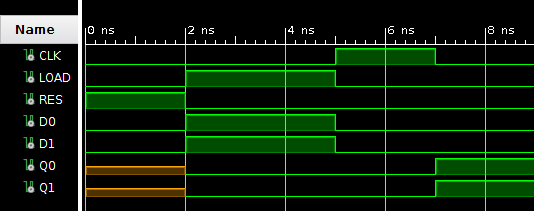
\includegraphics[width=\textwidth]{reg2_waveform.png}
    \caption[Verhalten des 2-Bit-Registers]{Zu Beginn wird das Register über
             das \texttt{res}"=Signal zurückgesetzt. Dadurch werden zunächst die
             internen Signale\texttt{q0\_s} und \texttt{q1\_s}, sowie
             \SI{2}{\nano\second} später die Ausgangssignale \texttt{q0} und
             \texttt{q1} von ihrem undefinierten Zustand auf den Wert
             \glqq 0\grqq\ gesetzt. Dann wird \texttt{res} auf \glqq 0\grqq\
             gesetzt, während \texttt{load} sowie die Eingänge \texttt{d0} und
             \texttt{d1} mit \glqq 1\grqq\ belegt werden. Dadurch werden nach
             weiteren \SI{3}{\nano\second} die internen Signale \texttt{q0\_ns}
             und \texttt{q1\_ns} ebenfalls auf \glqq 1\grqq\ gesetzt. Durch das
             Anlegen der Taktflanke (\texttt{clk} = \glqq 1\grqq) nach insgesamt
             \SI{5}{\nano\second} übernehmen \texttt{q0\_s} und \texttt{q1\_s}
             die Werte von \texttt{q0\_ns} und \texttt{q1\_s}, was sich
             \SI{2}{\nano\second} später an den Ausgangssignalen zeigt.}
    \label{fpga:hdl:waveform}
\end{figure}

Der Prozess \texttt{mux} beschreibt eine kombinatorische Funktion. Er
nimmt die Signale \texttt{load}, \texttt{q0\_s}, \texttt{q1\_s},
\texttt{d0} sowie \texttt{d1} entgegen und gibt die Signale \texttt{q0\_ns} und
\texttt{q1\_ns} aus. Ist \texttt{load} logisch \glqq 1\grqq\, werden \texttt{d0}
und \texttt{d1} ausgegeben, ansonsten die gespeicherten Signale \texttt{q0\_s}
und \texttt{q1\_s}. In Moore"=Schaltwerk aus Abbildung~\ref{fpga:hdl:moore}
entspricht \texttt{mux} somit der Eingabe"=Transferfunktion.
\cite[vgl.][31]{kesel2013}

Die Ausgabe"=Transferfunktion ist in diesem Beispiel als impliziter Prozess
dargestellt: \texttt{q0} und \texttt{q1} sind die Ausgabe $Y$ des
Moore"=Schaltwerks und wurden einfach mit den internen Signalen \texttt{q0\_s}
und \texttt{q1\_s} verbunden.
\cite[vgl.][31]{kesel2013}

Prozesse sind in VHDL als Modellierungen realer Hardware zu verstehen. So lässt
sich für das oben entworfene 2"=Bit"=Register eine äquivalente
Hardware"=Schaltung aus zwei Multiplexern und zwei taktflankengesteuerten
D"=Flip"=Flops mit asynchronen Set- und Reset-Eingängen aufbauen, wie Kesel und
Bartholomä zeigen \cite[siehe][32]{kesel2013}. Die im Prozess \texttt{reg}
verwendeten Signale \texttt{q0\_s} und \texttt{q1\_s} entsprechen dabei den
Flip"=Flops, während die Multiplexer den \texttt{mux}"=Prozess implementieren.
\cite[vgl.][31]{kesel2013}


\begin{code}
    \begin{minted}[fontsize=\small]{vhdl}
ARCHITECTURE beh OF reg2 IS
    SIGNAL q0_s, q0_ns, q1_s, q1_ns : std_logic;
BEGIN
    reg: PROCESS (clk, res)
    BEGIN
        IF res = '1' THEN
            q0_s <= '0';
            q1_s <= '0';
        ELSIF clk'event AND clk = '1' THEN
            q0_s <= q0_ns;
            q1_s <= q1_ns;
        END IF;
    END PROCESS reg;

    q0 <= q0_s AFTER 2 ns;
    q1 <= q1_s AFTER 2 ns;

    mux: PROCESS (load, q0_s, q1_s, d0, d1)
    BEGIN
        IF load = '1' THEN
            q0_ns <= d0 AFTER 3 ns;
            q1_ns <= d1 AFTER 3 ns;
        ELSE
            q0_ns <= q0_s AFTER 4 ns;
            q1_ns <= q1_s AFTER 4 ns;
        END IF;
    END PROCESS mux;
END beh;
    \end{minted}
    \caption{Verhaltensbeschreibung eines 2-Bit-Registers \cite[siehe][28]{kesel2013}}
    \label{fpga:hdl:regbeh}
\end{code}

\subsubsection{Strukturbeschreibungen}

Eine Strukturbeschreibung (auch Netzliste genannt) besteht aus mehreren
Teil-Komponenten, die zu einer größeren, komplexeren Komponente 
zusammengeschaltet werden. So lässt sich für die aus den vorherigen Abschnitten
bekannte \texttt{reg2}"=\textit{Entity} aus einem Modell eines Multiplexers
sowie einem Modell eines Flip"=Flops zusammensetzen (siehe
Quelltext~\ref{fpga:hdl:regstruct}\footnote{Die Verhaltensbeschreibungen der
Komponenten \texttt{mux2} und \texttt{ff2} sind in
Anhang~\ref{anhang:source:vhdl} zu finden.}).

Wie bei der Verhaltensbeschreibung gibt es auch bei der Strukturbeschreibung
Ports, das heißt von außen ein- bzw.\ nach außen ausgehende Signale, sowie
interne Signale für die Kommunikation der Teil-Komponenten untereinander. Die
einzelnen Komponenten werden zunächst mit ihren lokalen Ports deklariert
(\texttt{COMPONENT}"=Abschnitte) und danach instanziiert; \texttt{I1} und
\texttt{I0} sind dabei Bezeichnungen für eine \textit{Instanz} der jeweiligen
\textit{Entity}. In der \texttt{PORT MAP} werden die Ports und Signale der
Komponente den lokalen Ports der Teil-Komponenten zugeordnet.
\cite[vgl.][37]{kesel2013}

\begin{code}
    \begin{minted}[fontsize=\small]{vhdl}
ARCHITECTURE struct of reg2
    SIGNAL o1          : std_logic;
    SIGNAL o2          : std_logic;
    SIGNAL q0_internal : std_logic;
    SIGNAL q1_internal : std_logic;

    COMPONENT ff2
    PORT (
        clk : IN    std_logic;
        d0  : IN    std_logic;
        d1  : IN    std_logic;
        res : IN    std_logic;
        q0  : OUT   std_logic;
        q1  : OUT   std_logic
    );
    END COMPONENT;
    COMPONENT mux2
    PORT (
        a1  : IN    std_logic;
        a2  : IN    std_logic;
        b1  : IN    std_logic;
        b2  : IN    std_logic;
        sel : IN    std_logic;
        o1  : OUT   std_logic;
        o2  : OUT   std_logic
    );
    END COMPONENT;

BEGIN

    I1  : ff2
        PORT MAP(
            clk => clk, d0 => o1, d1 => o2,
            res => res, q0 => q0_internal, q1 => q1_internal
        );
    I0  : mux2
        PORT MAP(
            a1 => d0, a2 => d1, b1 => q0_internal,
            b2 => q1_internal, sel => load, o1 => o1, o2 => o2
        );

    q0 <= q0_internal;
    q1 <= q1_internal;

END struct;
    \end{minted}
    \caption{Strukturbeschreibung eines 2-Bit-Registers \cite[siehe][36]{kesel2013}}
    \label{fpga:hdl:regstruct}
\end{code}
\noindent

\subsubsection{Weitere Konzepte}

Die hier vorgestellten Konzepte einer Hardware"=Beschreibungssprache bilden nur
einen sehr geringen Teil der zur Verfügung stehenden Möglichkeiten ab. Neben den
gezeigten Grundbausteinen verfügen VHDL und Verilog noch über weitergehende
Fähigkeiten, wie etwa Verzweigungen, Schleifen, Operatoren und deren Überladung
oder rudimentäre Objektorientierung. Aufgrund der Zielsetzung dieser Arbeit kann
hier nicht weiter darauf eingegangen werden. Eine sehr gute Einführung in die
Programmierung mit VHDL ist aber bei Kesel und Bartholomä zu finden
\cite[siehe][]{kesel2013}. 

\subsubsection{Nebenläufigkeit}

Einer der wesentlichen Unterschiede zwischen VHDL und Hochsprachen, die auf
der algorithmischen Ebene arbeiten, ist die von vornherein vorhandene
Nebenläufigkeit. Während Befehle in C++ nacheinander abgearbeitet werden, gilt
dies bei VHDL nur innerhalb eines \textit{Prozesses}. \textit{Prozesse} arbeiten
unabhängig voneinander und werden nur über ihre Eingangssignale gesteuert, was
sich so auch auf die reale Hardware abbilden lässt. \cite[vgl.][25]{kesel2013}

\subsection{High-Level-Synthese und Parallelität}\label{fpga:entwicklung:hls}

Aus den im vorherigen Abschnitt gezeigten Beispielen wird schnell ersichtlich,
dass der Entwurf komplexerer Schaltungen mit einem hohen Konzeptions- und
Arbeitsaufwand verbunden ist und nicht nur gute Kenntnisse des  abzubildenden
Algorithmus erfordert, sondern darüber hinaus auch Wissen über die
Digitaltechnik verlangt. Mit der High"=Level"=Synthese (HLS) gibt es einen
Ansatz, die konkrete Schaltung durch Abstraktion zu verbergen und sich dem
Programmiermodell anderer Hardware"=Typen (\gls{cpu}s, \gls{gpu}s) anzunähern.
Bei der HLS findet der Entwurf vollständig auf der algorithmischen oder
Systemebene statt. Anschließend wird aus dem erzeugten Modell durch
HLS"=Werkzeuge ein Modell auf der Register"=Transfer"=Ebene erzeugt, aus dem im
nächsten Schritt die konkrete Schaltung synthetisiert werden kann. Auf
herkömmliche Programmiersprachen übertragen entspricht der Entwurf mit einer
Hardware"=Beschreibungssprache also der Programmierung einer \gls{cpu} mit einer
Assemblersprache.
\cite[vgl.][7]{hlsintro2019}

Während des algorithmischen Entwurfs kann der Nutzer zudem Randbedingungen
festlegen, die die HLS steuern, wie z.B. den angestrebten Ressourcenbedarf,
den gewünschten Datendurchsatz, \textit{Pipelining} oder die
Konfiguration des BlockRAMs. Bei der Erzeugung des Register"=Transfer"=Modells
werden diese Randbedingungen dann von den HLS"=Werkzeugen berücksichtigt.
\cite[vgl.][482]{kesel2013}

Die HLS wird zur Zeit von einigen Herstellern für mehrere Programmiersprachen
bzw. Erweiterungen bestehender Programmiersprachen unterstützt. Der Hersteller
Xilinx bietet beispielsweise HLS"=Werkzeuge für die Sprachen C, C++ und SystemC
an und unterstützt darüber hinaus den \gls{opencl}"=Standard. Einen ähnlichen
Weg geht die Firma Intel, die HLS"=Werkzeuge für C und C++ sowie \gls{opencl}
anbietet.

Die folgenden Erläuterungen richten sich nach den Handbüchern des Herstellers
Xilinx, die zugrunde liegenden Konzepte gelten jedoch für alle \gls{fpga}s.

\subsubsection{Scheduling}

\gls{fpga}s sind inhärent parallel. Anweisungen, die von einem bestimmten
Hardware"=Abschnitt ausgeführt werden (in VHDL durch \textit{Prozesse}
modelliert), sind sequentiell, während unterschiedliche Hardware"=Abschnitte in
Bezug aufeinander nebenläufig sind. Diese Eigenschaft unterscheidet \gls{fpga}s
deutlich von Prozessorarchitekturen, wie das folgende Beispiel zeigt.

Jeder Prozessor führt ein Programm als eine Folge von Instruktionen aus. Diese
Instruktionen werden von Compilern aus einer Hochsprache wie C++ in eine
prozessorspezifische Assemblersprache übersetzt:
\begin{code}
    \begin{minted}[fontsize=\small]{c++}
z = a + b;
    \end{minted}
\end{code}
wird wie folgt transformiert:
\begin{code}
    \begin{minted}[fontsize=\small]{gas}
movl    -8(%rbp), %edx
movl    -4(%rbp), %edx
addl    %edx, %eax
movl    %eax, -12(%rbp)
    \end{minted}
\end{code}
Selbst eine relativ simple Operation wie die Addition zweier Zahlen resultiert
in vier sequentiell auszuführenden Maschineninstruktionen. Je nachdem, wo die
Operanden liegen oder wo das Ergebnis gespeichert werden soll, können die
Instruktionen für Laden und Speichern (im Verhältnis zur Addition) viele
Taktzyklen benötigen. \cite[vgl.][18]{hlsintro2019}

Soll die Addition für viele Elemente ausgeführt werden, wie zum Beispiel in
einer Schleife, müssen diese vier Instruktionen stets wiederholt werden, da sich
alle Operationen dieselbe \gls{alu} teilen.

Bei der HLS kann diese Operation auf Hardware abgebildet werden, die
ausschließlich für diese Operation verwendet wird. Wenn \texttt{a}, \texttt{b}
und \texttt{z} \SI{32}{\bit} groß sind, wird dieser Datentyp durch 32 \gls{lut}
implementiert\footnote{Eine LUT entspricht einer Wahrheitstabelle für ein Bit.}.
Im Gegensatz zu Prozessoren werden bei einer \gls{fpga}"=Implementierung für
jede Operation innerhalb des Algorithmus voneinander unabhängige
\gls{lut}"=Mengen instanziiert.
\cite[vgl.][19]{hlsintro2019}

Eine Schleife ließe sich auf \gls{fpga}s also ganz oder teilweise ausrollen und,
sofern zwischen den einzelnen Iterationen keine Abhängigkeiten bestehen,
parallel ausführen. Die während der HLS vorgenommene Analyse der Daten- und
Kontrollflussabhängigkeiten wird im \gls{fpga}"=Kontext als Scheduling
bezeichnet. \cite[vgl.][19]{hlsintro2019}

\subsubsection{Pipelining-Prinzip}

Das von Prozessoren bekannte Prinzip des \textit{Pipelinings} findet bei
\gls{fpga}s ebenfalls Anwendung. Dabei werden Datenabhängigkeiten so aufgeteilt,
dass die ursprüngliche Verarbeitungsreihenfolge beibehalten wird, während die
benötigten Hardware"=Einheiten in eine Verkettung unabhängiger Stufen unterteilt
werden. Jede Stufe erhält ihre Eingangsdaten von der vorherigen Stufe und reicht
ihr Teilergebnis an die nächste Stufe weiter. Beispielsweise lässt sich die
folgende Funktion auf einen Multiplizierer und zwei Addierer abbilden:
\[
    y = (a \cdot x) + b + c
\]
Die resultierende Hardware"=Schaltung ist in
Abbildung~\ref{fpga:pipelining:schaltung} dargestellt. Die obere Schaltung
berechnet $y$ ohne Pipelining, die untere Schaltung zeigt die transformierte
Schaltung mit Pipelining.
\begin{figure}[htb]
    \centering
    \begin{tikzpicture}
        % untere Schaltung
        % a
        \draw (0.2, 5.15) -- (0.4, 5.35) node [pos = 1.0, xshift = 1.2mm, yshift = 2mm] {$a$};
        \draw (0, 5.25) -- (0.75, 5.25);
        \draw [thick, fill = HKS92!50] (0.75, 5) rectangle (1.25, 5.5);
        \draw [-{Latex}] (1.25, 5.25) -- (2.25, 5.25) -- (2.25, 4.75);

        % x
        \draw (0.2, 2.65) -- (0.4, 2.85) node [pos = 1.0, xshift = 1.2mm, yshift = 2mm] {$x$};
        \draw (0, 2.75) -- (0.75, 2.75);
        \draw [thick, fill = HKS92!50] (0.75, 2.5) rectangle (1.25, 3);
        \draw [-{Latex}] (1.25, 2.75) -- (2.25, 2.75) -- (2.25, 3.25);

        % b
        \draw (0.2, 1.4) -- (0.4, 1.6) node [pos = 1.0, xshift = 1.2mm, yshift = 2mm] {$b$};
        \draw (0, 1.5) -- (0.75, 1.5);
        \draw [thick, fill = HKS92!50] (0.75, 1.25) rectangle (1.25, 1.75);
        \draw (1.25, 1.5) -- (3.5, 1.5);
        \draw [thick, fill = HKS92!50] (3.5, 1.25)  rectangle (4, 1.75);
        \draw [-{Latex}] (4, 1.5) -- (6, 1.5) -- (6, 2);

        % c
        \draw (0.2, 0.15) -- (0.4, 0.35) node [pos = 1.0, xshift = 1.2mm, yshift = 2mm] {$c$};
        \draw (0, 0.25) -- (0.75, 0.25);
        \draw [thick, fill = HKS92!50] (0.75, 0) rectangle (1.25, 0.5);
        \draw (1.25, 0.25) -- (3.5, 0.25);
        \draw [thick, fill = HKS92!50] (3.5, 0) rectangle (4, 0.5);
        \draw [-{Latex}] (4, 0.25) -- (8.75, 0.25) -- (8.75, 0.75);

        % Multiplizierer
        \draw [thick] (2.25, 4) circle [radius = 0.75] node {\textbf{*}};
        \draw (3.0, 4) -- (3.5, 4);
        \draw [thick, fill = HKS92!50] (3.5, 3.75) rectangle (4, 4.25);
        \draw [-{Latex}] (4, 4) -- (6, 4) -- (6, 3.5);

        % erster Addierer
        \draw [thick] (6, 2.75) circle [radius = 0.75] node {\textbf{+}};
        \draw [-{Latex}] (6.75, 2.75) -- (8.75, 2.75) -- (8.75, 2.25);

        % zweiter Addierer
        \draw [thick] (8.75, 1.5) circle [radius = 0.75] node {\textbf{+}}; 

        % y
        \draw (9.5, 1.5) -- (10.25, 1.5);
        \draw [thick, fill = HKS92!50] (10.25, 1.25) rectangle (10.75, 1.75);
        \draw [-{Latex}] (10.75, 1.5) -- (11.5, 1.5);
        \draw (11.0, 1.4) -- (11.2, 1.6) node [pos = 1.0, xshift = 1.2mm, yshift = 2mm] {$y$};

        % Pfeil
        \draw (6, 5.75) -- ++(135:0.71) 
                        -- ++(0.25,0) 
                        -- ++(0, 0.75) 
                        -- ++(0.5, 0) 
                        -- ++(0, -0.75) node [right, xshift = 3mm] {\small Pipeline-Transformation}
                        -- ++(0.25, 0) 
                        -- ++(-135:0.71);

        % obere Schaltung
        % a
        \draw (0.2, 12.65) -- (0.4, 12.85) node [pos = 1.0, xshift = 1.2mm, yshift = 2mm] {$a$};
        \draw [-{Latex}] (0, 12.75) -- (2.25, 12.75) -- (2.25, 12.25);

        % x
        \draw (0.2, 10.15) -- (0.4, 10.35) node [pos = 1.0, xshift = 1.2mm, yshift = 2mm] {$x$};
        \draw [-{Latex}] (0, 10.25) -- (2.25, 10.25) -- (2.25, 10.75);

        % b
        \draw (0.2, 8.9) -- (0.4, 9.1) node [pos = 1.0, xshift = 1.2mm, yshift = 2mm] {$b$};
        \draw [-{Latex}] (0, 9) -- (6, 9) -- (6, 9.5);

        % c
        \draw (0.2, 7.65) -- (0.4, 7.85) node [pos = 1.0, xshift = 1.2mm, yshift = 2mm] {$c$};
        \draw [-{Latex}] (0, 7.75) -- (8.75, 7.75) -- (8.75, 8.25);

        % Multiplizierer
        \draw [thick] (2.25, 11.5) circle [radius = 0.75] node {\textbf{*}};
        \draw [-{Latex}] (3, 11.5) -- (6, 11.5) -- (6, 11);

        % erster Addierer
        \draw [thick] (6, 10.25) circle [radius = 0.75] node {\textbf{+}};
        \draw [-{Latex}] (6.75, 10.25) -- (8.75, 10.25) -- (8.75, 9.75);

        % zweiter Addierer
        \draw [thick] (8.75, 9) circle [radius = 0.75] node {\textbf{+}}; 

        % y
        \draw [-{Latex}] (9.5, 9) -- (11.5, 9);
        \draw (11.0, 8.9) -- (11.2, 9.1) node [pos = 1.0, xshift = 1.2mm, yshift = 2mm] {$y$};
    \end{tikzpicture}
    \caption{FPGA"=Implementierung einer mehrstufigen Berechnung \cite[nach][21]{hlsintro2019}}
    \label{fpga:pipelining:schaltung}
\end{figure}
\noindent
Die grauen Kästen der unteren Schaltung entsprechen Registern, die in realer
Hardware durch Flip"=Flops realisiert werden. Jeder Kasten kann dabei als ein
zusätzlicher Taktzyklus aufgefasst werden. Die Berechnung eines einzelnen
Ergebnisses benötigt dadurch drei zusätzliche Taktzyklen. Durch die zusätzlichen
Register lassen sich die einzelnen Schritte der Berechnung jedoch in unabhängige
Abschnitte aufteilen, der Multiplizierer und die Addierer können also
nebenläufig arbeiten. Die Ergebnisse $y$ und $y'$ lassen sich auf diese Weise
(teilweise) parallel berechnen und lasten dabei die verfügbare Hardware besser
aus: Nach einem Overhead von 3 Taktzyklen zu Beginn der Berechnung (engl.
\textit{pipeline fill time}) berechnet die Schaltung in jedem weiteren
Taktzyklus einen neuen Wert für $y$. Dieser Vorgang wird in
Abbildung~\ref{fpga:pipelining:pipeline} illustriert. Je nach verwendetem
Algorithmus ist es möglich, dass die Pipeline nicht in jedem Taktzyklus eine
neue Schleifeniteration verarbeiten kann (z.B. aufgrund bestehender
Abhängigkeiten zwischen einzelnen Iterationen). Die Anzahl der Zyklen, die
zwischen dem Beginn zweier aufeinanderfolgender Iterationen liegen, werden als
\gls{ii} bezeichnet. Wenn $\text{II} = 1$ gilt, beginnt die Pipeline mit
jedem Takt eine neue Schleifeniteration. Bei $\text{II} = 2$ schafft sie dies
nur alle zwei Takte, bei $\text{II} = 4$ mit jedem vierten Takt, usw.
\cite[vgl.][20--21]{hlsintro2019}

\begin{figure}[htb]
    \centering
    \begin{tikzpicture}
        % a
        \draw (0.2, 5.15) -- (0.4, 5.35) node [pos = 1.0, xshift = 1.2mm, yshift = 2mm] {$a$};
        \draw (0, 5.25) -- (0.75, 5.25);
        \draw [thick, fill = HKS92!75] (0.75, 5) rectangle (1.25, 5.5);
        \draw [-{Latex}] (1.25, 5.25) -- (2.25, 5.25) -- (2.25, 4.75);

        % x
        \draw (0.2, 2.65) -- (0.4, 2.85) node [pos = 1.0, xshift = 1.2mm, yshift = 2mm] {$x$};
        \draw (0, 2.75) -- (0.75, 2.75);
        \draw [thick, fill = HKS92!75] (0.75, 2.5) rectangle (1.25, 3);
        \draw [-{Latex}] (1.25, 2.75) -- (2.25, 2.75) -- (2.25, 3.25);

        % b
        \draw (0.2, 1.4) -- (0.4, 1.6) node [pos = 1.0, xshift = 1.2mm, yshift = 2mm] {$b$};
        \draw (0, 1.5) -- (0.75, 1.5);
        \draw [thick, fill = HKS92!75] (0.75, 1.25) rectangle (1.25, 1.75);
        \draw (1.25, 1.5) -- (3.5, 1.5);
        \draw [thick] (3.5, 1.25) rectangle (4, 1.75);
        \draw [-{Latex}] (4, 1.5) -- (6, 1.5) -- (6, 2);

        % c
        \draw (0.2, 0.15) -- (0.4, 0.35) node [pos = 1.0, xshift = 1.2mm, yshift = 2mm] {$c$};
        \draw (0, 0.25) -- (0.75, 0.25);
        \draw [thick, fill = HKS92!75] (0.75, 0) rectangle (1.25, 0.5);
        \draw (1.25, 0.25) -- (3.5, 0.25);
        \draw [thick] (3.5, 0) rectangle (4, 0.5);
        \draw [-{Latex}] (4, 0.25) -- (8.75, 0.25) -- (8.75, 0.75);

        % Multiplizierer
        \draw [thick] (2.25, 4) circle [radius = 0.75] node {\textbf{*}};
        \draw (3.0, 4) -- (3.5, 4);
        \draw [thick] (3.5, 3.75) rectangle (4, 4.25);
        \draw [-{Latex}] (4, 4) -- (6, 4) -- (6, 3.5);

        % erster Addierer
        \draw [thick, fill = HKS92!50] (6, 2.75) circle [radius = 0.75] node {\textbf{+}};
        \draw [-{Latex}] (6.75, 2.75) -- (8.75, 2.75) -- (8.75, 2.25);

        % zweiter Addierer
        \draw [thick, fill = HKS92!50] (8.75, 1.5) circle [radius = 0.75] node {\textbf{+}}; 

        % y
        \draw (9.5, 1.5) -- (10.25, 1.5);
        \draw [thick, fill = HKS92!50] (10.25, 1.25) rectangle (10.75, 1.75);
        \draw [-{Latex}] (10.75, 1.5) -- (11.5, 1.5);
        \draw (11.0, 1.4) -- (11.2, 1.6) node [pos = 1.0, xshift = 1.2mm, yshift = 2mm] {$y$};

        % Formeln
        \draw [thick, fill = HKS92!75] (-1, -3.5) rectangle (1.35, -0.5)
              node [pos = 0.5, align = center, text = white] { $a(i)$ \\ 
                                                               $x(i)$ \\ 
                                                               $b(i)$ \\ 
                                                               $c(i)$ };
        \draw [thick] (1.35, -3.5) rectangle (4.5, -0.5)
              node [pos = 0.5, align = center] { $a(i - 1) \cdot x(i - 1)$ \\
                                                 $b(i - 1)$ \\
                                                 $c(i - 1)$};
        \draw [thick, fill = HKS92!50] (4.5, -3.5) rectangle (11.5, -0.5)
              node [pos = 0.5, align = center] { $(a(i - 2) \cdot x(i - 2)) + b(i - 2) + c(i - 2)$};
    \end{tikzpicture}
    \caption{FPGA"=Pipeline"=Architektur \cite[nach][22]{hlsintro2019}}
    \label{fpga:pipelining:pipeline}
\end{figure}

Die Anwendung des Pipelining während der HLS unterscheidet sich zwischen den
Herstellern: So versucht Intels OpenCL"=Umgebung grundsätzlich, Pipelining auf
jede vorhandene Schleife anzuwenden und erfordert ein explizites Deaktivieren
des Verfahrens, wenn kein Pipelining gewünscht wird. Bei Xilinx'
OpenCL"=Umgebung verhält es sich dagegen genau umgekehrt, da hier Pipelining
explizit angeschaltet werden muss.

\subsubsection{Producer-Consumer-Prinzip}

Neben dem Pipelining gibt es auf \gls{fpga}s eine weitere Möglichkeit,
Parallelität auszudrücken. Diese ähnelt dem Pipelining-Prinzip, arbeitet jedoch
auf einer groberen Ebene. Dahinter steht das Ziel, diese Funktionen
weitestgehend parallel auszuführen. Dazu analysieren die HLS"=Werkzeuge die Ein- 
und Ausgangsparameter der im Algorithmus vorhandenen Funktionen. Im einfachsten
Fall gibt es keine gemeinsam bearbeiteten Daten, wodurch alle Funktionen
parallel ausgeführt werden können. Naturgemäß ist dieser Fall recht selten,
üblicherweise werden die Ergebnisse einer Funktion von einer oder mehreren
nachfolgenden Funktionen verarbeitet. Dieses als
\textit{Producer"=Consumer}"=Prinzip bekannte Verfahren kann durch die
Nebenläufigkeit der FPGA"=Hardware parallelisiert werden. Durch den Einsatz von
Block RAM als FIFO"=Puffer zwischen den Hardware"=Abschnitten, die aus der
jeweiligen Funktion synthetisiert wurden, kann die produzierende Funktion
während ihrer Ausführung Teilergebnisse speichern. Die konsumierende Funktion
kann diese Teilergebnisse nach der initialen Wartezeit, die ebenfalls als
\gls{ii} bezeichnet wird, direkt weiter verarbeiten, ohne auf das Ende der
produzierenden Funktion bzw.\ das resultierende Gesamtergebnis warten zu müssen.
\cite[vgl.][22--23]{hlsintro2019}

Das Producer"=Consumer"=Prinzip wird je nach Hersteller unterschiedlich benannt.
So nennt sich dieses Verfahren bei Xilinx \textit{Dataflow}, während es bei
Intel \textit{Channel} heißt.
